\documentclass[a4paper, 12pt, conference, portuguese]{ieeeconf}

\IEEEoverridecommandlockouts
\overrideIEEEmargins
\usepackage{graphics}
\usepackage{epsfig}
\usepackage{mathptmx}
\usepackage{times}
\usepackage{amsmath}
\usepackage{amssymb}
\usepackage[left=3cm,right=3cm,top=3cm,bottom=3cm]{geometry}
\usepackage[utf8]{inputenc}
\usepackage[portuguese]{babel}

\title{{\LARGE \bf Cálculo de Sub-Redes e Pontos de Articulação}
\large{Relatório do 1º Projecto - Análise e Síntese de Algoritmos} }

\author{Baltasar Dinis, 89416 e Afonso Ribeiro, 86752}

\begin{document}
\maketitle
\thispagestyle{empty}
\pagestyle{empty}

\begin{abstract}
  Uma rede deve ser desenhada de forma a que seja resiliente a falhas de
  componentes individuais, permitindo ao seu utilizador uma utilização contínua
  do sistema. A existência de pontos únicos de falha\footnote{\textit{Single
  Points of Failure} em inglês} compromete esta resiliência, impedindo que a
  rede consiga escalar face ao tráfego. Neste relatório, expomos uma
  metodologia para automaticamente verificar se uma rede é resiliente e quantas
  sub-redes estão presentes na mesma. Este trabalho foi realizado no contexto da
  Unidade Curricular de Análise e Síntese de Algoritmos, no ano lectivo de
  2018-2019.
\end{abstract}



\section{INTRODUÇÃO}\label{intro}
Redes de computadores são hoje em dia ubíquas e essenciais para o funcionamento
normal de empresas, do Estado e da sociedade em geral. Devido à sua importância,
uma rede deve ser capaz de tolerar falhas individuais e independentes dos seus
componentes, de forma a que um serviço que a utilize consiga escalar com o
tráfego. Se a rede tiver um ponto que, ao falhar, desconecte a rede, não se pode considerar que a rede tem uma topologia
resiliente. É por isso importante conseguir, de forma expedita, identificar
estes pontos.

É também útil conseguir saber quais são as sub-redes existentes numa dada
topologia de roteadores, e o que aconteceria caso esses pontos falhassem
simultaneamente.

Neste relatório, apresentaremos uma solução para este problema. A estrutura
do relatório é a seguinte: em \ref{sol},
fazemos um mapeamento do problema para um problema de grafos e
expomos a nossa solução; em \ref{theoric}, fazemos uma análise teórica do
algoritmo empregue, nomeadamente em termos de complexidade; em
\ref{experimental} apresentamos os resultados da nossa avaliação experimental e
em \ref{conclusion} comentamos a correspondência entre os resultados
experimentais e os valores teóricos.

\section{DESCRIÇÃO DA SOLUÇÃO}\label{sol}
Representamos uma rede de roteadores como um grafo não dirigido. Notemos que uma
sub-rede é uma componente do grafo, pois existem caminhos entre dois quaisquer
roteadores de uma sub-rede, e não existe nenhum roteador atingível a partir de
um outro na sub-rede que não pertença ele mesmo à sub-rede.

Mapeamos conceptualmente os pontos únicos de falha na noção de ponto de
articulação. Na literatura, \cite{cormen}, define-se um ponto de articulação como
aquele cuja remoção causaria uma desconexão de um grafo conexo (consideramos as
componentes como sub-grafos conexos). Note-se a seguinte, e interessante,
propriedade dos pontos de articulação:

\textbf{Lema.} Seja ${\cal G} = ({\cal V}, {\cal E})$ um grafo e $a \in {\cal
V}$. Se existir um par
de vértices $u, v \in {\cal V}$ tal que existe um caminho de $u$ para $v$ que passa por
$a$. Então $a$ é um ponto de
articulação se e só se todos os caminhos de $u$ para $v$ passarem por $a$.

\textbf{Dem.} Se existir um caminho de $u$ para $v$ que não passe por $a$ então
a remoção de $a$ não faz com que a componente se desconecte. Se $a$ é um ponto
de articulação então a sua remoção terá de desconectar a componente. Isto só
acontece se todos os caminhos que vão de $u$ para $v$ passarem por $a$ (caso
contrário a componente manter-se-ia conexa).

Note-se que esta propriedade é importante ( em \cite{tarjan1} é dada como a
definição de ponto de articulação) definindo a essência do ponto de
articulação como ponto único de falha.

A nossa abordagem baseia-se na procura em
profundidade\footnote{\textit{Depth-First Search}, ou DFS, em inglês}, empregando algoritmos
definidos por Tarjan \cite{tarjan1}, \cite{tarjan2}. Em cada uma das subsecções
seguintes apresentamos como a DFS é aplicada para produzir cada um dos

\subsection{Cálculo de Sub-Redes}
Uma sub-rede é uma componente do grafo. Como descrito em \cite{tarjan2}, podemos
obter as componentes aplicando a DFS. A partir de um vértice qualquer, começamos
a fazer a procura. Quando não existirem mais vértices a
explorar encontramos todos os vértices da componente.

No contexto do problema, não temos que
identificar a componente inteira, mas sim o identificador do roteador com maior
índice.  Fazemos isso de forma eficiente impondo uma ordenação na extracção.
Extraímos o roteador não visitado de maior índice, adicionando-o ao fim de uma
lista que guarda os identificadores das sub-redes, pois é garantido que todos os
roteadores de índice maior que o dele já tenham sido explorados - não sendo
possível que façam parte desta componente.

Como temos de imprimir a lista de identificadores de sub-rede por ordem crescente,
percorremos a lista em ordem inversa.

\subsection{Cálculo de Pontos de Articulação}\label{art}
Introduzimos os seguintes lemas .

\textbf{Lema.} Se $v \in {\cal V}$ tiver menos de duas adjacências não é um ponto
de articulação. A demonstração é trivial.

\textbf{Lema.} Seja $root \in {\cal V}$ a raiz de uma árvore gerada pela DFS.
$root$ é um ponto de articulação se e só se tem pelo menos duas crianças na árvore.

\textbf{Dem.} Se não tiver pelo menos duas adjacências (pelo lema anterior) não
pode ser ponto de articulação. Se tiver $n$ crianças é
garantido que não hajam ligações entre as sub-árvores (se existissem, não seriam
sub-árvores distintas, pois só se escolhe o filho da raiz após a árvore estar
completamente explorada). Logo a raiz tem de ser o único nó a ligar as
sub-árvores, sendo um ponto de articulação.

\textbf{Def. } (Aresta para Trás) Dizemos que $(u, v)$ é uma aresta para trás
numa DFS quando tanto $u$ como $v$ já foram descobertos, $u$ é descendente de
$v$ e está a ser tratada a aresta.

Para calcular as arestas para trás, mantemos uma lista dos valores de $low:
{\cal V} \to \mathbb{N}$, para além da usual lista de valores de descoberta
($d$) e de pais ($\pi$).
$low(v)$ é o mínimo entre o tempo da sua descoberta e
o $low$ dos seus descendentes directos. Isto significa que, se existir uma aresta
para trás $(u, w)$, onde $u$ é descendente de $v$ e $w$ antecessor, então
$low(u) = low(w)$. Assim, conseguimos descobrir se um dos filhos de $v$ (ou algum dos seus
descendentes) tem arestas para um dos antecessores de $v$.

Podemos sintetizar dois predicados, um para dados dois vértices descobrir se
existe uma aresta para trás (e subsequentemente actualizar o $low$) e outro
para, dada uma sub-árvore DFS (completamente explorada), descobrir se há uma
aresta para trás da raiz da sub-árvore.
\begin{align*}
  is\_back\_edge(u, w) \leftarrow \\ d(w) < d(u) \land \pi(u) \neq w \\
  subtree\_has\_backedge(root) \leftarrow \\ \exists c \in Children(root) : \\
  low(c) < low(root)
\end{align*}

Com base nisto, podemos verificar se um ponto é de articulação ou não utilizando
o seguinte predicado.
\begin{align*}\label{predicate}
  is\_articulation\_point(v) \leftarrow \\ (is\_dfs\_root(v) \land n\_children(v) \geq
  2) \lor \\ (\lnot is\_dfs\_root(v) \land  \exists u \in Children(v) : \\ \lnot subtree\_has\_backedge(u))
\end{align*}

Fazemos este cálculo para todos os nós à medida que se faz a pesquisa (mantendo uma
estrutura de booleanos que indica se eles são pontos de articulação), calculando o
predicado se o nó ainda não for ponto de articulação.

\subsection{Componente Máxima}\label{dfs}
Depois de remover os nós (marcando-os com uma cor especial), calculamos uma
versão simplificada da DFS, onde mantemos apenas o tamanho da maior componente.

\section{ANÁLISE TEÓRICA}\label{theoric}

A nossa implementação tem 4 passos relevantes:
\begin{enumerate}
  \item
    Construir o grafo;
  \item
    Aplicar uma DFS, como descrito em \ref{art} para calcular os pontos de
    articulação;
  \item
    Remover os pontos de articulação;
  \item
    Tornar a aplicar uma DFS, como descrito em \ref{dfs}, para calcular o
    tamanho da maior sub-rede.
\end{enumerate}

Notemos que, uma vez calculados os pontos de articulação, removê-los é uma
operação trivial, completada em $\Theta(V)$, no pior caso (basta marcá-los com uma
cor especial).

\subsection{Representação do Grafo}
Representamos o grafo por uma lista de adjacências. Notemos que esta
representação é $O(V + E)$ \cite{cormen} em uso de memória e que a operação de obter a lista
e adjacências de um nó é $O(1)$.

\subsection{Construção do Grafo}
O input é dado em $3$ secções: 1) Uma linha com o número de roteadores; 2) Uma
linha com o número de ligações; 3) lista de ligações. Logo a leitura é feita em
$\Theta(E)$.

Como a adição de um nó no grafo é executada em tempo constante e a adição de uma
aresta também, concluímos que a construção do grafo é $\Theta(V + E)$.

\subsection{Pesquisa em Profundidade}
Aplicar uma DFS é tem complexidade temporal $\Theta(V + E)$ \cite{cormen}.
Mostramos agora que a nossas adaptações da pesquisa limitam-se a fazer computações
em tempo constante, e que por isso o nosso algoritmo adaptado é também um $\Theta(V + E)$.

Na primeira aplicação, que calcula os pontos de articulação e os identificadores
das sub-redes, são feitas as seguintes operações:
\begin{itemize}
  \item Inicializações: $\Theta(1)$
  \item Obtenção da lista nós adjacentes: $\Theta(1)$\\

  Para cada adjacente não descoberto
  \item Incrementação do número de filhos: $\Theta(1)$
  \item Inicialização do valor do pai: $\Theta(1)$
  \item Actualização do $low$ (comparação e eventual atribuição) : $\Theta(1)$
  \item Verificação se é ponto de articulação : $\Theta(1)$, pois as
    dependências do predicado apresentado em \ref{art} já se encontram
    calculadas, ou são calculáveis em $\Theta(1)$ \\

  Para cada adjacente (fora o pai) não descoberto:
  \item Actualização do $low$: $\Theta(1)$
\end{itemize}

\newpage
Na segunda aplicação a visita é mais simples:
\begin{itemize}
  \item Inicialização da cor: $\Theta(1)$
  \item Obtenção da lista nós adjacentes: $\Theta(1)$\\ \\
  Para cada adjacente não descoberto
  \item Incrementação do número de nós da sub-rede: $\Theta(1)$
\end{itemize}

Como todas as operações da visita não estruturais à pesquisa em profundidade são
$\Theta(1)$ e a própria pesquisa é $\Theta(V + E)$, concluímos que ambas as
aplicações têm uma complexidade $\Theta(V + E)$.

\subsection{Avaliação do Algoritmo Proposto}
Concluímos que o algoritmo tem complexidade:
\begin{align*}
  &\Theta(V + E) && \tag{Construção do Grafo}\\
  + &\Theta(V + E) && \tag{Aplicação 1ª DFS}\\
  + &\Theta(V) && \tag{Rem. P. de Articulação}\\
  + &\Theta(V + E) && \tag{Aplicação 2ª DFS}\\
  = 3&\Theta(V + E) + \Theta(V)
  = &\Theta(V + E)
\end{align*}

\section{AVALIAÇÃO EXPERIMENTAL}\label{experimental}
Para a avaliação experimental, geramos testes com as seguintes variantes.
\begin{itemize}
  \item V: número de roteadores na rede
  \item E: número de ligações na rede
  \item S: número de sub-redes
\end{itemize}

Consideramos mais interessante o caso onde $E > V$, pois no caso contrário há
pelo menos $V - (2 * E)$ vértices sozinhos. Desta forma, conseguimos redes mais
complexas e, por conseguinte, aplicações não triviais do algoritmo.

\begin{figure}[t]
  \centering
  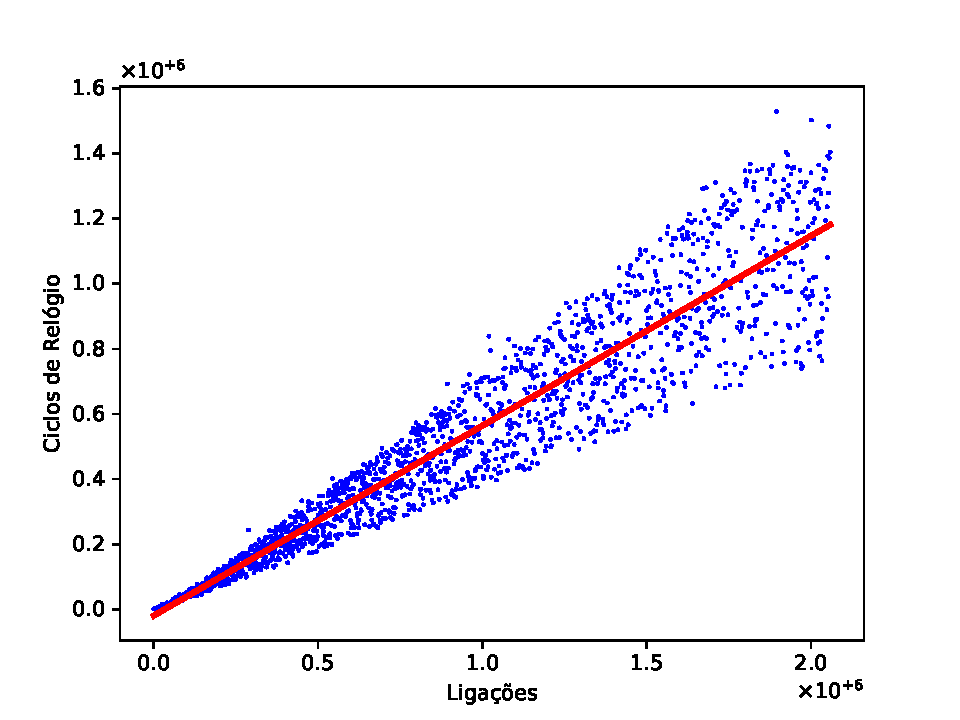
\includegraphics[width=1.0\linewidth]{analysis}
  \caption{Resultados experimentais: Latência em função do número de arestas}
  \label{res}
\end{figure}

Na Figura \ref{res} está exposta a relação entre o número de arestas e a
complexidade temporal (medida em número de ciclos de relógio). A recta de
regressão linear encontrada tem um coeficiente de determinação $R^2 = 0.897$,
pelo que concluímos que o desempenho da nossa solução varia linearmente com o
número de arestas do grafo, estando por isso em concordância com a análise
teórica.

Os testes foram efectuados numa arquitectura Intel$^\circledR$ Core\texttrademark
i5-6200U. O código foi instrumentado directamente, através da inclusão de duas
instruções, uma para obter o valor do relógio no momento inicial e outra no
momento final.

\section{CONCLUSÃO}\label{conclusion}

Apresentámos uma solução para o problema de descoberta de pontos de falha única
numa rede, bem como uma simulação do pior caso para a rede - a falha simultânea de
todos os pontos de falha única. Para tal, mapeamos o problema para um problema
de grafos, onde procuramos os pontos de articulação. Para tal, recorremos a uma variante da
pesquisa em profundidade. Para calcular o tamanho da maior componente,
limitamo-nos a aplicar de novo a pesquisa em profundidade. Mostramos
teoricamente e confirmamos experimentalmente esses resultados, onde conseguimos
que a solução tivesse complexidade $\Theta(V + E)$.

\begin{thebibliography}{99}
  \bibitem{cormen} T. Cormen, C. Leiserson e L. R. Rivest, \textit{Introduction
    to Algorithms} 1ª edição. Cambridge, Massachussets: The MIT Press,
    1990.
  \bibitem{tarjan1} R. E. Tarjan. ``Depth-First Search and Linear Graph
    Algorithms'' in SIAM Journal on Computing, Vol. 1, No. 2, June 1972.
  \bibitem{tarjan2} J. Hopcroft and R. E. Tarjan. ``Efficient Algorithms for
    Graph Manipulation'' in Communications of the ACM, Vol. 16, No. 6, 1973.
\end{thebibliography}
\end{document}
